\usetikzlibrary{arrows,decorations.markings}

\def\dirxx{1}
\def\dirxy{0.2}
\def\diryx{0.4}
\def\diryy{0.7}

\def\dirax{0.2}
\def\diray{0.04}
\def\dirorthax{0.05}
\def\dirorthay{-0.25}
\def\dirbx{0.12}
\def\dirby{0.21}
\def\dirorthbx{-0.21}
\def\dirorthby{0.12}
\def\dircx{0.2}
\def\dircy{-0.16666}
\def\dirorthcx{0.16666}
\def\dirorthcy{0.2}

\def\specialbox{
  
          \foreach \x/\y in {0.5/0, 1.5/0, 2.5/0, 3.5/0}
          {
            \draw[thick,draw=white,-{Latex[length=1.4mm]}, >=stealth]
            (\x*\dirxx+\y*\diryx+2*\dirorthax-1.2*\dirax,\x*\dirxy+\y*\diryy+2*\dirorthay-1.2*\diray) --
            (\x*\dirxx+\y*\diryx+2*\dirorthax+1.4*\dirax,\x*\dirxy+\y*\diryy+2*\dirorthay+1.4*\diray) ;
          }

          \foreach \x/\y in {0/0.5, 0/1.5, 0/2.5, 0/3.5}
          {
            \draw[thick,draw=white,-{Latex[length=1.4mm]}, >=stealth]
            (\x*\dirxx+\y*\diryx+2*\dirorthbx-1.2*\dirbx,\x*\dirxy+\y*\diryy+2*\dirorthby-1.2*\dirby) --
            (\x*\dirxx+\y*\diryx+2*\dirorthbx+1.4*\dirbx,\x*\dirxy+\y*\diryy+2*\dirorthby+1.4*\dirby) ;
          }

          \foreach \x/\y in {3.5/0.5, 2.5/1.5, 1.5/2.5, 0.5/3.5}
          {
            \draw[thick,draw=white,-{Latex[length=1.4mm]}, >=stealth]
            (\x*\dirxx+\y*\diryx+2*\dirorthcx-1.2*\dircx,\x*\dirxy+\y*\diryy+2*\dirorthcy-1.2*\dircy) --
            (\x*\dirxx+\y*\diryx+2*\dirorthcx+1.4*\dircx,\x*\dirxy+\y*\diryy+2*\dirorthcy+1.4*\dircy) ;
          }
}

\def\eps{0.22}
\def\ax{0.4}
\def\ay{0.4}

\newcommand\drawuvdivfreedof[4]{
  %\draw[#4] ({#1+#3*\eps},{#2}) arc[start angle=0, end angle=360, x radius={#3*\eps}, y radius={#3*\eps}];
  \draw[->,>=stealth,#4] ({#1+#3*\eps},{#2}) arc[start angle=0, end angle=315, x radius={#3*\eps}, y radius={#3*\eps}];
}

\newcommand\drawuvpdivfreedof[3]{
  \draw[draw=#3,fill=#3,opacity=0.15] (#1,#2) circle [radius=0.2] ;
  \draw[->,>=stealth,#3] (#1+0.2,#2) arc[start angle=0, end angle=315, x radius=0.2, y radius=0.2];
  \draw[draw=#3,fill=#3] (#1,#2) circle [radius=0.08cm] ;
}

\newcommand\drawuvdof[4]{
  \draw[#4,-{Latex[length=0.9mm]}, >=stealth] ({#1+0.05*#3},{#2}) -- ({#1+0.3*#3},{#2});
  \draw[#4,-{Latex[length=0.9mm]}, >=stealth] ({#1},{#2+0.05*#3}) -- ({#1},{#2+0.3*#3});
}

\newcommand\drawpdof[3]{
  \draw[draw=#3,fill=#3] (#1,#2) circle [radius=0.08cm] ;
}

\begin{figure}
  \centering
  \resizebox{0.99\linewidth}{!}{
    \begin{tabular}{c@{~}c@{\hspace*{-0.4cm}}c@{\hspace*{-0.3cm}}c@{\hspace*{-0.3cm}}c@{\hspace*{-0.3cm}}c@{\hspace*{-0.15cm}}c@{\hspace*{-0.2cm}}c}
      &
        Trefftz-DG
      &
        DG
      &
        Solenoidal DG
      &
        $H(\Div)$-DG
      &
        $H(\Div)$-HDG
      &
      Rhebergen-Wells-HDG
      &
        Taylor--Hood
      \\
      &
        $\IT^4$
      &
        $[\IP^{4}]^2/\IP^3$
      &
        \makecell{$[\IP^4]^2\!\cap\!\{\Div v\!=\!0\}/\!$\\ $\IP^4(\Fh)$}
      &
        $\BDM^{4}/\IP^3$
      &
        $\BDM^{4}/\IP^{3}_\tau(\Fh)/\IP^{3}$
      &
      \makecell{$[\IP^4]^2\!/[\IP^4]^2(\Fh)/$\\ $\IP^4(\Fh)$}      
      &
        $[\IP^4\!\cap\!C^0]^2\!/(\IP^3\!\cap\!C^0)$
      \\[1ex]
      \rotatebox{90}{\hspace*{0.6cm}velocity}
      &
      \multirow{2}{*}{
\parbox{0.2\linewidth}{\vspace{-2em}
        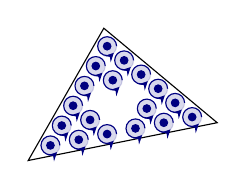
\begin{tikzpicture}[scale=0.6]
          % \tikz
          \def\dirxx{1}
          \def\dirxy{0.2}
          \def\diryx{0.4}
          \def\diryy{0.7}


          \draw (0,0) -- (4*\dirxx,4*\dirxy) -- (4*\diryx,4*\diryy) -- cycle;


          \foreach \x/\y in { 
            0.3/0.3, 0.9/0.3, 1.5/0.3, 2.1/0.3, 2.7/0.3, 3.3/0.3,
            0.3/0.9, 0.9/0.9,          2.1/0.9, 2.7/0.9,
            0.3/1.5,                   2.1/1.5,
            0.3/2.1, 0.9/2.1, 1.5/2.1,
            0.3/2.7, 0.9/2.7,
            0.3/3.3
          }
          % \foreach \x/\y in { 0.70588/0.70588, 
          %     1.64706/0.70588, 
          %     2.58824/0.70588,
          %     0.70588/1.64706,
          %     1.64706/1.64706,
          %     0.70588/2.58824
          % }
          {
            \drawuvpdivfreedof{0.05+\x*\dirxx+\y*\diryx}{0.05+\x*\dirxy+\y*\diryy}{blue!50!black}
          }
        \end{tikzpicture}
}}
      &
        \begin{tikzpicture}[scale=0.6]
          % \tikz

          \def\ax{0.35}
          \def\ay{0.35}
          
          \specialbox
          
          \draw (0,0) -- (4*\dirxx,4*\dirxy) -- (4*\diryx,4*\diryy) -- cycle;

          \foreach \x/\y in {0/0, 1/0, 2/0, 3/0, 4/0,
            0/1, 3/1,
            0/2, 2/2,
            0/3, 1/3,
            0/4,
            1/1,2/1,1/2}
          {
              \drawuvdof{((1-0.3)*\x+0.3*1.35)*\dirxx+((1-0.3)*\y+0.3*1.35)*\diryx}{((1-0.3)*\x+0.3*1.35)*\dirxy+((1-0.3)*\y+0.3*1.35)*\diryy}{1.0}{blue!50!black}
          }
        \end{tikzpicture}
      &
        \begin{tikzpicture}[scale=0.6]
          % \tikz
          \def\dirxx{1}
          \def\dirxy{0.2}
          \def\diryx{0.4}
          \def\diryy{0.7}

          \specialbox

          \draw (0,0) -- (4*\dirxx,4*\dirxy) -- (4*\diryx,4*\diryy) -- cycle;

          \foreach \x/\y in {
            0.5/0.5, 1.0/0.5, 1.5/0.5, 2.0/0.5, 2.5/0.5, 3.0/0.5,
            0.5/1.0, 1.0/1.0, 1.5/1.0, 2.0/1.0, 2.5/1.0, 
            0.5/1.5, 1.0/1.5, 1.5/1.5, 2.0/1.5, 
            0.5/2.0, 1.0/2.0, %1.5/2.0, 
            0.5/2.5, 1.0/2.5,
            0.5/3.0            
            }
          {
            \drawuvdivfreedof{\x*\dirxx+\y*\diryx}{\x*\dirxy+\y*\diryy}{0.7}{blue!50!black}
          }
        \end{tikzpicture}
      &
        \begin{tikzpicture}[scale=0.6]
          % \tikz

          \def\ax{0.2}
          \def\ay{0.2}

          \specialbox

          \draw (0,0) -- (4*\dirxx,4*\dirxy) -- (4*\diryx,4*\diryy) -- cycle;
          
          \foreach \x/\y in {0.66666/0, 1.33333/0, 2/0, 2.66666/0, 3.33333/0}
          {
            \draw[thick,draw=blue!50!black,fill=blue!50!black,-{Latex[length=1.4mm]}, >=stealth]
            (\x*\dirxx+\y*\diryx-\dirorthax,\x*\dirxy+\y*\diryy-\dirorthay) --
            (\x*\dirxx+\y*\diryx+\dirorthax,\x*\dirxy+\y*\diryy+\dirorthay) ;
          }

          \foreach \x/\y in {0/0.66666, 0/1.33333, 0/2, 0/2.66666, 0/3.33333}
          {
            \draw[thick,draw=blue!50!black,fill=blue!50!black,-{Latex[length=1.4mm]}, >=stealth]
            (\x*\dirxx+\y*\diryx-\dirorthbx,\x*\dirxy+\y*\diryy-\dirorthby) --
            (\x*\dirxx+\y*\diryx+\dirorthbx,\x*\dirxy+\y*\diryy+\dirorthby) ;
          }

          \foreach \x/\y in {3.33333/0.66666, 2.66666/1.33333, 2/2, 1.33333/2.66666, 0.66666/3.33333}
          {
            \draw[thick,draw=blue!50!black,fill=blue!50!black,-{Latex[length=1.4mm]}, >=stealth]
            (\x*\dirxx+\y*\diryx-\dirorthcx,\x*\dirxy+\y*\diryy-\dirorthcy) --
            (\x*\dirxx+\y*\diryx+\dirorthcx,\x*\dirxy+\y*\diryy+\dirorthcy) ;
          }

          \foreach \x/\y in {1/1, 2/1,
            1/2}
          {
            % \draw[draw=blue!50!black,fill=blue!50!black] (\x*\dirxx+\y*\diryx,\x*\dirxy+\y*\diryy) circle [radius=0.08cm] ;
          }

          \foreach \x/\y in {1.64706/0.70588,
            1.17647/1.17647, 1.64706/1.17647,
            0.70588/1.64706, 1.17647/1.64706, 1.64706/1.64706}
          {
            \draw[draw=blue!50!black,fill=blue!50!black] (\x*\dirxx+\y*\diryx,\x*\dirxy+\y*\diryy) circle [radius=0.08cm] ;
          }

          \foreach \x/\y in {0.70588/0.70588, 1.17647/0.70588, 2.11765/0.70588, 2.58824/0.70588,
            0.70588/1.17647, 2.11765/1.17647,
            0.70588/2.11765, 1.17647/2.11765,
            0.70588/2.58824}
          {
            \draw[draw=red!80!black] (\x*\dirxx+\y*\diryx,\x*\dirxy+\y*\diryy) circle [radius=0.08cm] ;
          }
        \end{tikzpicture}

      &
        \vspace*{0.4cm}
        \begin{tikzpicture}[scale=0.6]
          % \tikz
          \def\dirxx{1}
          \def\dirxy{0.2}
          \def\diryx{0.4}
          \def\diryy{0.7}

          \def\dirax{0.2}
          \def\diray{0.04}
          \def\dirorthax{0.05}
          \def\dirorthay{-0.25}
          \def\dirbx{0.12*0.75}
          \def\dirby{0.21*0.75}
          \def\dirorthbx{-0.21}
          \def\dirorthby{0.12}
          \def\dircx{0.2*0.75}
          \def\dircy{-0.16666*0.75}
          \def\dirorthcx{0.16666}
          \def\dirorthcy{0.2}

          \def\ax{0.2}
          \def\ay{0.2}

          \draw (0,0) -- (4*\dirxx,4*\dirxy) -- (4*\diryx,4*\diryy) -- cycle;

          \foreach \x/\y in {0.66666/0, 1.33333/0, 2/0, 2.66666/0, 3.33333/0}
          {
            \draw[thick,draw=blue!50!black,fill=blue!50!black,-{Latex[length=1.4mm]}, >=stealth]
            (\x*\dirxx+\y*\diryx-\dirorthax,\x*\dirxy+\y*\diryy-\dirorthay) --
            (\x*\dirxx+\y*\diryx+\dirorthax,\x*\dirxy+\y*\diryy+\dirorthay) ;
          }
          \foreach \x/\y in {0.5/0, 1.5/0, 2.5/0, 3.5/0}
          {
            \draw[thick,draw=blue!50!black,fill=blue!50!black,-{Latex[length=1.4mm]}, >=stealth]
            (\x*\dirxx+\y*\diryx+2*\dirorthax-1.2*\dirax,\x*\dirxy+\y*\diryy+2*\dirorthay-1.2*\diray) --
            (\x*\dirxx+\y*\diryx+2*\dirorthax+1.4*\dirax,\x*\dirxy+\y*\diryy+2*\dirorthay+1.4*\diray) ;
          }

          \foreach \x/\y in {0/0.66666, 0/1.33333, 0/2, 0/2.66666, 0/3.33333}
          {
            \draw[thick,draw=blue!50!black,fill=blue!50!black,-{Latex[length=1.4mm]}, >=stealth]
            (\x*\dirxx+\y*\diryx-\dirorthbx,\x*\dirxy+\y*\diryy-\dirorthby) --
            (\x*\dirxx+\y*\diryx+\dirorthbx,\x*\dirxy+\y*\diryy+\dirorthby) ;
          }

          \foreach \x/\y in {0/0.5, 0/1.5, 0/2.5, 0/3.5}
          {
            \draw[thick,draw=blue!50!black,fill=blue!50!black,-{Latex[length=1.4mm]}, >=stealth]
            (\x*\dirxx+\y*\diryx+2*\dirorthbx-1.2*\dirbx,\x*\dirxy+\y*\diryy+2*\dirorthby-1.2*\dirby) --
            (\x*\dirxx+\y*\diryx+2*\dirorthbx+1.4*\dirbx,\x*\dirxy+\y*\diryy+2*\dirorthby+1.4*\dirby) ;
          }

          \foreach \x/\y in {3.33333/0.66666, 2.66666/1.33333, 2/2, 1.33333/2.66666, 0.66666/3.33333}
          {
            \draw[thick,draw=blue!50!black,fill=blue!50!black,-{Latex[length=1.4mm]}, >=stealth]
            (\x*\dirxx+\y*\diryx-\dirorthcx,\x*\dirxy+\y*\diryy-\dirorthcy) --
            (\x*\dirxx+\y*\diryx+\dirorthcx,\x*\dirxy+\y*\diryy+\dirorthcy) ;
          }

          \foreach \x/\y in {3.5/0.5, 2.5/1.5, 1.5/2.5, 0.5/3.5}
          {
            \draw[thick,draw=blue!50!black,fill=blue!50!black,-{Latex[length=1.4mm]}, >=stealth]
            (\x*\dirxx+\y*\diryx+2*\dirorthcx-1.2*\dircx,\x*\dirxy+\y*\diryy+2*\dirorthcy-1.2*\dircy) --
            (\x*\dirxx+\y*\diryx+2*\dirorthcx+1.4*\dircx,\x*\dirxy+\y*\diryy+2*\dirorthcy+1.4*\dircy) ;
          }

          \foreach \x/\y in {1/1, 2/1,
            1/2}
          {
            % \draw[draw=blue!50!black,fill=blue!50!black] (\x*\dirxx+\y*\diryx,\x*\dirxy+\y*\diryy) circle [radius=0.08cm] ;
          }

          \foreach \x/\y in {1.64706/0.70588,
            1.17647/1.17647, 1.64706/1.17647,
            0.70588/1.64706, 1.17647/1.64706, 1.64706/1.64706}
          {
            \draw[draw=green!50!black] (\x*\dirxx+\y*\diryx,\x*\dirxy+\y*\diryy) circle [radius=0.08cm] ;
          }

          \foreach \x/\y in {0.70588/0.70588, 1.17647/0.70588, 2.11765/0.70588, 2.58824/0.70588,
            0.70588/1.17647, 2.11765/1.17647,
            0.70588/2.11765, 1.17647/2.11765,
            0.70588/2.58824}
          {
            \draw[draw=red!80!black] (\x*\dirxx+\y*\diryx,\x*\dirxy+\y*\diryy) circle [radius=0.08cm] ;
          }

            \draw[draw=black,very thin]
            (0.0*\dirxx+0.0*\diryx+2*\dirorthax,0.0*\dirxy+0.0*\diryy+2*\dirorthay) --
            (4.0*\dirxx+0.0*\diryx+2*\dirorthax,4.0*\dirxy+0.0*\diryy+2*\dirorthay);
            \draw[draw=black,very thin]
            (0.0*\dirxx+0.0*\diryx+2*\dirorthbx,0.0*\dirxy+0.0*\diryy+2*\dirorthby) --
            (0.0*\dirxx+4.0*\diryx+2*\dirorthbx,0.0*\dirxy+4.0*\diryy+2*\dirorthby);
            \draw[draw=black,very thin]
            (4.0*\dirxx+0.0*\diryx+2*\dirorthcx,4.0*\dirxy+0.0*\diryy+2*\dirorthcy) --
            (0.0*\dirxx+4.0*\diryx+2*\dirorthcx,0.0*\dirxy+4.0*\diryy+2*\dirorthcy);
        \end{tikzpicture}
      &
      \vspace*{0.4cm} %sasdf
      \begin{tikzpicture}[scale=0.6]
        % \tikz
        \def\dirxx{1}
        \def\dirxy{0.2}
        \def\diryx{0.4}
        \def\diryy{0.7}

        \def\dirax{0.2}
        \def\diray{0.04}
        \def\dirorthax{0.05}
        \def\dirorthay{-0.25}
        \def\dirbx{0.12*0.75}
        \def\dirby{0.21*0.75}
        \def\dirorthbx{-0.21}
        \def\dirorthby{0.12}
        \def\dircx{0.2*0.75}
        \def\dircy{-0.16666*0.75}
        \def\dirorthcx{0.16666}
        \def\dirorthcy{0.2}

        \def\ax{0.2}
        \def\ay{0.2}

        \draw (0,0) -- (4*\dirxx,4*\dirxy) -- (4*\diryx,4*\diryy) -- cycle;

        \foreach \x/\y in {3.6/0.4, 2.8/1.2, 2.0/2.0, 1.2/2.8, 0.4/3.6}
        {
          \drawuvdof{\x*\dirxx+\y*\diryx+2*\dirorthcx}{\x*\dirxy+\y*\diryy+2*\dirorthcy}{1.0}{blue!50!black}
        }

        \foreach \x/\y in {0/0.4, 0/1.2, 0/2.0, 0/2.8, 0/3.6}
        {
          \drawuvdof{\x*\dirxx+\y*\diryx+2*\dirorthbx}{\x*\dirxy+\y*\diryy+2*\dirorthby}{1.0}{blue!50!black}
        }

        \foreach \x/\y in {0.4/0, 1.2/0, 2.0/0, 2.8/0, 3.6/0}
        {
          \drawuvdof{\x*\dirxx+\y*\diryx+2*\dirorthax}{\x*\dirxy+\y*\diryy+2*\dirorthay}{1.0}{blue!50!black}
        }


        \foreach \x/\y in {1/1, 2/1,
          1/2}
        {
          % \draw[draw=blue!50!black,fill=blue!50!black] (\x*\dirxx+\y*\diryx,\x*\dirxy+\y*\diryy) circle [radius=0.08cm] ;
        }

        \foreach \x/\y in {
          0.5/0.5, 1.0/0.5, 1.5/0.5, 2.0/0.5, 2.5/0.5, 3.0/0.5,
          0.5/1.0, 1.0/1.0, 1.5/1.0, 2.0/1.0, 2.5/1.0, 
          0.5/1.5, 1.0/1.5, 1.5/1.5, 2.0/1.5, 
          0.5/2.0, 1.0/2.0, 1.5/2.0, 
          0.5/2.5, 1.0/2.5,
          0.5/3.0            
          }
        {
          \drawuvdof{\x*\dirxx+\y*\diryx}{\x*\dirxy+\y*\diryy}{0.925}{green!50!black}
        }


          \draw[draw=black,very thin]
          (0.0*\dirxx+0.0*\diryx+2*\dirorthax,0.0*\dirxy+0.0*\diryy+2*\dirorthay) --
          (4.0*\dirxx+0.0*\diryx+2*\dirorthax,4.0*\dirxy+0.0*\diryy+2*\dirorthay);
          \draw[draw=black,very thin]
          (0.0*\dirxx+0.0*\diryx+2*\dirorthbx,0.0*\dirxy+0.0*\diryy+2*\dirorthby) --
          (0.0*\dirxx+4.0*\diryx+2*\dirorthbx,0.0*\dirxy+4.0*\diryy+2*\dirorthby);
          \draw[draw=black,very thin]
          (4.0*\dirxx+0.0*\diryx+2*\dirorthcx,4.0*\dirxy+0.0*\diryy+2*\dirorthcy) --
          (0.0*\dirxx+4.0*\diryx+2*\dirorthcx,0.0*\dirxy+4.0*\diryy+2*\dirorthcy);
      \end{tikzpicture}
    &
        \begin{tikzpicture}[scale=0.6]
          % \tikz

          \def\ax{0.35}
          \def\ay{0.35}
          
          \specialbox
          
          \draw (0,0) -- (4*\dirxx,4*\dirxy) -- (4*\diryx,4*\diryy) -- cycle;

          
          \foreach \x/\y in {0/0, 1/0, 2/0, 3/0, 4/0,
            0/1, 1/1, 2/1, 3/1,
            0/2, 1/2, 2/2,
            0/3, 1/3,
            0/4}
          {
          }

          \foreach \x/\y in {1/1, 2/1,
            1/2}
          {
            \drawuvdof{\x*\dirxx+\y*\diryx}{\x*\dirxy+\y*\diryy}{1.0}{green!50!black}
          }

          \foreach \x/\y in {0/0, 1/0, 2/0, 3/0, 4/0,
            0/1, 3/1,
            0/2, 2/2,
            0/3, 1/3,
            0/4}
          {
            \drawuvdof{\x*\dirxx+\y*\diryx}{\x*\dirxy+\y*\diryy}{1.0}{blue!50!black}
          }
        \end{tikzpicture}
        \vspace*{-0.6cm}
      \\
      %
      %
      %
      %
      %
      %
      %
      %
      %
      %
      %
      %
      %
      %
      %
      %
      %
      %
      \rotatebox{90}{\hspace*{0.4cm}pressure}
      &
      &
        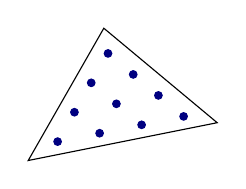
\begin{tikzpicture}[scale=0.6]
          % \tikz
          \def\dirxx{1}
          \def\dirxy{0.2}
          \def\diryx{0.4}
          \def\diryy{0.7}

          \def\ax{0.2}
          \def\ay{0.2}

          \draw (0,0) -- (4*\dirxx,4*\dirxy) -- (4*\diryx,4*\diryy) -- cycle;

          \foreach \x/\y in {1.33333/1.33333, 0.44444/0.44444, 1.33333/0.44444, 2.22222/0.44444, 3.11111/0.44444,
            0.44444/1.33333, 2.22222/1.33333,
            0.44444/2.22222, 1.33333/2.22222,
            0.44444/3.11111}
          {
            \draw[draw=blue!50!black,fill=blue!50!black] (\x*\dirxx+\y*\diryx,\x*\dirxy+\y*\diryy) circle [radius=0.08cm] ;
          }

        \end{tikzpicture} 
      &
        \vspace*{0.4cm}
        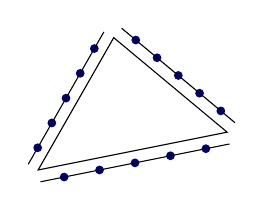
\begin{tikzpicture}[scale=0.6]
          % \tikz
          \def\dirxx{1}
          \def\dirxy{0.2}
          \def\diryx{0.4}
          \def\diryy{0.7}

          \def\dirax{0.2}
          \def\diray{0.04}
          \def\dirorthax{0.05}
          \def\dirorthay{-0.25}
          \def\dirbx{0.12}
          \def\dirby{0.21}
          \def\dirorthbx{-0.21}
          \def\dirorthby{0.12}
          \def\dircx{0.2}
          \def\dircy{-0.16666}
          \def\dirorthcx{0.16666}
          \def\dirorthcy{0.2}

          \def\ax{0.2}
          \def\ay{0.2}

          \draw (0,0) -- (4*\dirxx,4*\dirxy) -- (4*\diryx,4*\diryy) -- cycle;

          \foreach \x/\y in {0.5/0, 1.25/0, 2.0/0, 2.75/0, 3.5/0}
          {
            \draw[draw=blue!50!black,fill=blue!50!black] 
            (\x*\dirxx+\y*\diryx+\dirorthax,\x*\dirxy+\y*\diryy+\dirorthay) circle [radius=0.08cm] ;
          }

          \foreach \x/\y in {0/0.5, 0/1.25, 0/2.0, 0/2.75, 0/3.5}
          {
            \draw[draw=blue!50!black,fill=blue!50!black] 
                (\x*\dirxx+\y*\diryx+\dirorthbx,\x*\dirxy+\y*\diryy+\dirorthby) circle [radius=0.08cm] ;
          }

          \foreach \x/\y in {3.5/0.5, 2.75/1.25, 2.0/2.0, 1.25/2.75, 0.5/3.5}
          {
            \draw[draw=blue!50!black,fill=blue!50!black] 
            (\x*\dirxx+\y*\diryx+\dirorthcx,\x*\dirxy+\y*\diryy+\dirorthcy) circle [radius=0.08cm] ;
            %(\x*\dirxx+\y*\diryx+2*\dirorthcx+1.4*\dircx,\x*\dirxy+\y*\diryy+2*\dirorthcy+1.4*\dircy) ;
          }

            \draw[draw=black]
            (0.0*\dirxx+0.0*\diryx+\dirorthax,0.0*\dirxy+0.0*\diryy+\dirorthay) --
            (4.0*\dirxx+0.0*\diryx+\dirorthax,4.0*\dirxy+0.0*\diryy+\dirorthay);
            \draw[draw=black]
            (0.0*\dirxx+0.0*\diryx+\dirorthbx,0.0*\dirxy+0.0*\diryy+\dirorthby) --
            (0.0*\dirxx+4.0*\diryx+\dirorthbx,0.0*\dirxy+4.0*\diryy+\dirorthby);
            \draw[draw=black]
            (4.0*\dirxx+0.0*\diryx+\dirorthcx,4.0*\dirxy+0.0*\diryy+\dirorthcy) --
            (0.0*\dirxx+4.0*\diryx+\dirorthcx,0.0*\dirxy+4.0*\diryy+\dirorthcy);
        \end{tikzpicture}
      &
        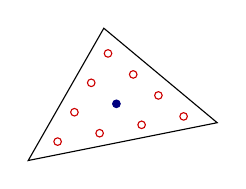
\begin{tikzpicture}[scale=0.6]
          % \tikz
          \def\dirxx{1}
          \def\dirxy{0.2}
          \def\diryx{0.4}
          \def\diryy{0.7}

          \def\ax{0.2}
          \def\ay{0.2}

          \draw (0,0) -- (4*\dirxx,4*\dirxy) -- (4*\diryx,4*\diryy) -- cycle;

          \foreach \x/\y in {0.44444/0.44444, 1.33333/0.44444, 2.22222/0.44444, 3.11111/0.44444,
            0.44444/1.33333, 1.33333/1.33333, 2.22222/1.33333,
            0.44444/2.22222, 1.33333/2.22222,
            0.44444/3.11111}
          {
          }

          \foreach \x/\y in {1.33333/1.33333}
          {
            \draw[draw=blue!50!black,fill=blue!50!black] (\x*\dirxx+\y*\diryx,\x*\dirxy+\y*\diryy) circle [radius=0.08cm] ;
          }

          \foreach \x/\y in {0.44444/0.44444, 1.33333/0.44444, 2.22222/0.44444, 3.11111/0.44444,
            0.44444/1.33333, 2.22222/1.33333,
            0.44444/2.22222, 1.33333/2.22222,
            0.44444/3.11111}
          {
            \draw[draw=red!80!black] (\x*\dirxx+\y*\diryx,\x*\dirxy+\y*\diryy) circle [radius=0.08cm] ;
          }
        \end{tikzpicture}
      &
        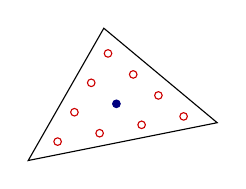
\begin{tikzpicture}[scale=0.6]
          % \tikz
          \def\dirxx{1}
          \def\dirxy{0.2}
          \def\diryx{0.4}
          \def\diryy{0.7}

          \def\ax{0.2}
          \def\ay{0.2}

          \draw (0,0) -- (4*\dirxx,4*\dirxy) -- (4*\diryx,4*\diryy) -- cycle;

          \foreach \x/\y in {0.44444/0.44444, 1.33333/0.44444, 2.22222/0.44444, 3.11111/0.44444,
            0.44444/1.33333, 1.33333/1.33333, 2.22222/1.33333,
            0.44444/2.22222, 1.33333/2.22222,
            0.44444/3.11111}
          {
          }

          \foreach \x/\y in {1.33333/1.33333}
          {
            \draw[draw=blue!50!black,fill=blue!50!black] (\x*\dirxx+\y*\diryx,\x*\dirxy+\y*\diryy) circle [radius=0.08cm] ;
          }

          \foreach \x/\y in {0.44444/0.44444, 1.33333/0.44444, 2.22222/0.44444, 3.11111/0.44444,
            0.44444/1.33333, 2.22222/1.33333,
            0.44444/2.22222, 1.33333/2.22222,
            0.44444/3.11111}
          {
            \draw[draw=red!80!black] (\x*\dirxx+\y*\diryx,\x*\dirxy+\y*\diryy) circle [radius=0.08cm] ;
          }
        \end{tikzpicture} 
      &
      \vspace*{0.4cm}
      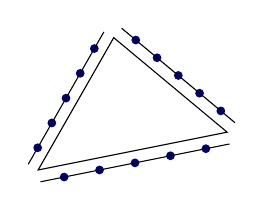
\begin{tikzpicture}[scale=0.6]
        % \tikz
        \def\dirxx{1}
        \def\dirxy{0.2}
        \def\diryx{0.4}
        \def\diryy{0.7}

        \def\dirax{0.2}
        \def\diray{0.04}
        \def\dirorthax{0.05}
        \def\dirorthay{-0.25}
        \def\dirbx{0.12}
        \def\dirby{0.21}
        \def\dirorthbx{-0.21}
        \def\dirorthby{0.12}
        \def\dircx{0.2}
        \def\dircy{-0.16666}
        \def\dirorthcx{0.16666}
        \def\dirorthcy{0.2}

        \def\ax{0.2}
        \def\ay{0.2}

        \draw (0,0) -- (4*\dirxx,4*\dirxy) -- (4*\diryx,4*\diryy) -- cycle;

        \foreach \x/\y in {0.5/0, 1.25/0, 2.0/0, 2.75/0, 3.5/0}
        {
          \draw[draw=blue!50!black,fill=blue!50!black] 
          (\x*\dirxx+\y*\diryx+\dirorthax,\x*\dirxy+\y*\diryy+\dirorthay) circle [radius=0.08cm] ;
        }

        \foreach \x/\y in {0/0.5, 0/1.25, 0/2.0, 0/2.75, 0/3.5}
        {
          \draw[draw=blue!50!black,fill=blue!50!black] 
              (\x*\dirxx+\y*\diryx+\dirorthbx,\x*\dirxy+\y*\diryy+\dirorthby) circle [radius=0.08cm] ;
        }

        \foreach \x/\y in {3.5/0.5, 2.75/1.25, 2.0/2.0, 1.25/2.75, 0.5/3.5}
        {
          \draw[draw=blue!50!black,fill=blue!50!black] 
          (\x*\dirxx+\y*\diryx+\dirorthcx,\x*\dirxy+\y*\diryy+\dirorthcy) circle [radius=0.08cm] ;
          %(\x*\dirxx+\y*\diryx+2*\dirorthcx+1.4*\dircx,\x*\dirxy+\y*\diryy+2*\dirorthcy+1.4*\dircy) ;
        }

          \draw[draw=black]
          (0.0*\dirxx+0.0*\diryx+\dirorthax,0.0*\dirxy+0.0*\diryy+\dirorthay) --
          (4.0*\dirxx+0.0*\diryx+\dirorthax,4.0*\dirxy+0.0*\diryy+\dirorthay);
          \draw[draw=black]
          (0.0*\dirxx+0.0*\diryx+\dirorthbx,0.0*\dirxy+0.0*\diryy+\dirorthby) --
          (0.0*\dirxx+4.0*\diryx+\dirorthbx,0.0*\dirxy+4.0*\diryy+\dirorthby);
          \draw[draw=black]
          (4.0*\dirxx+0.0*\diryx+\dirorthcx,4.0*\dirxy+0.0*\diryy+\dirorthcy) --
          (0.0*\dirxx+4.0*\diryx+\dirorthcx,0.0*\dirxy+4.0*\diryy+\dirorthcy);
      \end{tikzpicture}
      &
        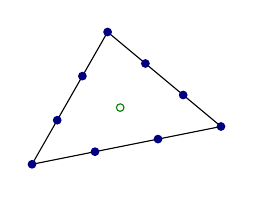
\begin{tikzpicture}[scale=0.6]
          % \tikz
          \def\dirxx{1}
          \def\dirxy{0.2}
          \def\diryx{0.4}
          \def\diryy{0.7}

          \def\ax{0.2}
          \def\ay{0.2}

          \draw (0,0) -- (4*\dirxx,4*\dirxy) -- (4*\diryx,4*\diryy) -- cycle;

          \foreach \x/\y in {0/0, 1.33333/0, 2.66666/0, 4/0,
            0/1.33333, 1.33333/1.33333, 2.66666/1.33333,
            0/2.66666, 1.33333/2.66666,
            0/4}
          {
          }

          \foreach \x/\y in {1.33333/1.33333}
          {
            \draw[draw=green!50!black] (\x*\dirxx+\y*\diryx,\x*\dirxy+\y*\diryy) circle [radius=0.08cm] ;
          }

          \foreach \x/\y in {0/0, 1.33333/0, 2.66666/0, 4/0,
            0/1.33333, 2.66666/1.33333,
            0/2.66666, 1.33333/2.66666,
            0/4}
          {
            \draw[draw=blue!50!black,fill=blue!50!black] (\x*\dirxx+\y*\diryx,\x*\dirxy+\y*\diryy) circle [radius=0.08cm] ;
          }
        \end{tikzpicture}
      \\[-1ex]
      \multicolumn{8}{c}{  \begin{tikzpicture}[scale=0.6]
          \drawuvdof{-16.1}{-0.2}{1.0}{black}
          \node[right] at (-16+0.1,-0.1) {\scriptsize ~\texttt{vel. \dofs} (\texttt{x} \& \texttt{y} \texttt{comp.s})} ;
          \drawpdof{-8}{-0.1}{black}
          \node[right] at (-8+0.1,-0.1) {\scriptsize ~\texttt{scalar} \dof} ;
          \drawuvdivfreedof{0}{-0.1}{0.7}{black}
          \node[right] at (0+0.1,-0.1) {\scriptsize ~\texttt{div-free} \texttt{vel.} \dof} ;
          \drawuvpdivfreedof{8}{-0.1}{black}
          \node[right] at (8+0.1,-0.1) {\scriptsize ~\texttt{Stokes} \texttt{vel./pr.} \dof} ;

          \node[scale=0.7,rectangle,draw,fill,blue!50!black] at (-16,-0.7){};
          \node[right] at (-16+0.1,-0.7) {\scriptsize ~\texttt{global} \dof} ;
          \node[scale=0.7,rectangle,draw,red!50!black] at (-8,-0.7){};
          \node[right] at (-8+0.1,-0.7) {\scriptsize ~\texttt{removable} \dof} ;
          \node[scale=0.7,rectangle,draw,green!50!black] at (0,-0.7){};
          \node[right] at (0+0.1,-0.7) {\scriptsize ~\texttt{locally condensable} \dof} ;
          % {\scriptsize ~global unknown} ;

          % \draw[-{Latex[length=1.4mm]}, >=stealth,blue!50!black] (0,-0.1) -- (0.35,-0.1) ;
          % \draw[-{Latex[length=1.4mm]}, >=stealth,blue!50!black] (0,-0.1) -- (0,0.25) ;
          % \draw[thick,draw=blue!50!black,fill=blue!50!black,-{Latex[length=1.4mm]}, >=stealth] (0.5,-0.2) -- (0.7,0.25) ;
          % \draw[draw=blue!50!black,fill=blue!80!black] (1,0) circle [radius=0.08cm] node[right] {\scriptsize ~global unknown} ;
          % \draw[-{Latex[length=1.4mm]}, >=stealth,green!50!black] (6,-0.1) -- (6.35,-0.1) ;
          % \draw[-{Latex[length=1.4mm]}, >=stealth,green!50!black] (6,-0.1) -- (6,0.25) ;
          % \draw[draw=green!50!black] (6.5,0) circle [radius=0.08cm] node[right] {\scriptsize ~local unknown (eliminable)} ;
          % \draw[draw=red!80!black] (14,0) circle [radius=0.08cm] node[right] {\scriptsize ~removable unknown } ;
        \end{tikzpicture}
      }
    \end{tabular}
}
  \caption{Sketch of fourth order FE discretisations with different types of unknowns for velocity and pressure: unknowns that can be removed beforehand if a suitable basis is used, local unknowns that can be eliminated by static condensation and the remaining global unknowns. Note that every arrow corresponds to one scalar \texttt{dof}.
  %The space $\protect\IP^{3}_\tau(\Fh)$ in the $H(\Div)$-HDG method is the space of vector-valued functions that are tangential polynomials up to degree three on every facet.
  }
  \label{fig:drawdofs}
\end{figure}

%%% Local Variables:
%%% mode: latex
%%% TeX-master: "SeMA-VMS-2017"
%%% End:
